\documentclass{beamer}

\usepackage{beamerthemesplit}
\usepackage{verbatim}

\usepackage{xcolor}

\definecolor{gold}{rgb}{1.,0.84,0.}
\definecolor{brightred}{rgb}{1.,0.4,0.4}
\definecolor{mygray}{RGB}{200,200,200}
\definecolor{lightsteelblue}{RGB}{176,196,222}
\definecolor{lightskyblue}{RGB}{135,206,250}
\definecolor{cadetblue}{RGB}{95,158,160}

\usetheme{default}
\usecolortheme{mule}

\usefonttheme{serif}

%\DeclareGraphicsExtensions{.pdf,.png,.jpg}

\newcommand{\snT}{$(S/N)_{\textrm{size}}$}
%\newcommand{\snT}{$\left( \frac{S}{N}\right)_{\textrm{size}}$}
\newcommand{\snflux}{$(S/N)_{\textrm{flux}}$}
%\newcommand{\snflux}{$\left( \frac{S}{N}\right)_{\textrm{flux}}$}

\newcommand{\lensfit}{\texttt{LENSFIT}}
\newcommand{\numba}{\texttt{Numba}}
\newcommand{\python}{\texttt{Python}}
\newcommand{\ngmix}{\texttt{ngmix}}
\newcommand{\shear}{{\bf g}}
\newcommand{\redmapper}{redMaPPer}

\newcommand{\prelim}{{\bf{\it Preliminary}}}



\title{Correction for Correlated Noise in Metacalibration}
\author{Erin Sheldon}
\institute{Brookhaven National Laboratory}

% http://texblog.net/latex-archive/plaintex/beamer-footline-frame-number/
% to add the page (frame ) number and not screw up the bottom line
% works for split themes?
\expandafter\def\expandafter\insertshorttitle\expandafter{%
      \insertshorttitle\hfill%
        \insertframenumber\,/\,\inserttotalframenumber}

% suppress navigation bar
\beamertemplatenavigationsymbolsempty
\setbeamertemplate{footline}{}

\begin{document}

\frame{\titlepage}


\setbeamertemplate{background canvas}[vertical shading][bottom=mgray,top=mblack]

\frame
{
    \frametitle{Outline}

    \setbeamerfont*{itemize/enumerate body}{size=\Large}
    \setbeamerfont*{itemize/enumerate subbody}{parent=itemize/enumerate body}
    \setbeamerfont*{itemize/enumerate subsubbody}{parent=itemize/enumerate body}
 
    \begin{itemize}

        %\item The Primary Goal is to Study Dark Energy
        \item Metacalibration

        \item Correlated Noise

        \item Correction for Correlated Noise

        \item Performance on Realistic Simulations

    \end{itemize}

}

\frame
{
    \frametitle{Shear Accuracy Requirements}

    \setbeamerfont*{itemize/enumerate body}{size=\Large}
    \setbeamerfont*{itemize/enumerate subbody}{parent=itemize/enumerate body}
    \setbeamerfont*{itemize/enumerate subsubbody}{parent=itemize/enumerate body}
 
    \begin{itemize}

        \item In order to measure the Dark Energy equation of state
            to the desired accuracy for DES/LSST, we must measure
            shear with exquisite accuracy.

        \item Shear calibration errors
            \begin{itemize}
            
                \item {\color{lightskyblue} DES}:~ $\Delta \gamma/\gamma \lesssim 0.004$
                \item {\color{brightred} LSST}: $\Delta \gamma/\gamma \lesssim 0.001$

            \end{itemize}


    \end{itemize}

}



\frame
{
    \frametitle{Metacalibration Idea from Eric Huff}

    \setbeamerfont*{itemize/enumerate body}{size=\normalsize}
    \setbeamerfont*{itemize/enumerate subbody}{parent=itemize/enumerate body}
    \setbeamerfont*{itemize/enumerate subsubbody}{parent=itemize/enumerate body}
 
    \begin{itemize}

        \item Say we have a biased shear estimator {\color{gold} $E$}.  Then we can write
            {\color{gold}
                \begin{eqnarray}
                    E & = & E(\gamma=0) + \frac{\partial E}{\partial \gamma} \gamma + ... \nonumber \\
                      & \sim &  \frac{\partial E}{\partial \gamma} \gamma \equiv R \gamma \nonumber 
                \end{eqnarray}
            } 
        \item Use image manipulation to estimate the derivative of the
            estimator with respect to shear
            {\color{gold}
                \begin{equation}
                    R = \frac{E(+\Delta\gamma) - E(-\Delta\gamma)}{2 \Delta \gamma} \nonumber 
                \end{equation}
            }
            \begin{itemize}
                \item Deconvolve the PSF
                \item Shear the image by a small amount
                \item Reconvolve by the PSF.  Use a slightly larger PSF to suppress
                    the noise amplification
            \end{itemize}


    \end{itemize}

}

\frame
{
    \frametitle{Metacalibration Idea from Eric Huff}

    \setbeamerfont*{itemize/enumerate body}{size=\Large}
    \setbeamerfont*{itemize/enumerate subbody}{parent=itemize/enumerate body}
    \setbeamerfont*{itemize/enumerate subsubbody}{parent=itemize/enumerate body}
 
    \begin{itemize}
        
        \item Should correct for modeling biases

        \item Should correct for {\em ordinary} noise-related biases

        \item Works well at high shear.

    \end{itemize}

}



\frame
{
    \frametitle{Correlated Noise}

    \setbeamerfont*{itemize/enumerate body}{size=\large}
    \setbeamerfont*{itemize/enumerate subbody}{parent=itemize/enumerate body}
    \setbeamerfont*{itemize/enumerate subsubbody}{parent=itemize/enumerate body}
 
    \begin{itemize}

        \item These convolutions and shears involved in the metacal process
            results in {\em {\color{gold} correlated noise}}
            
        \item Fluctuations due to noise are no longer independent after convolution.

        \item Fluctuations due to noise are no longer independent after shear, due
            to interpolation.

        \item Can result in bias of order $5-10$\% for very faint galaxies.


    \end{itemize}

}

\frame
{
    \frametitle{Correlated Noise Example}

    \begin{figure}
        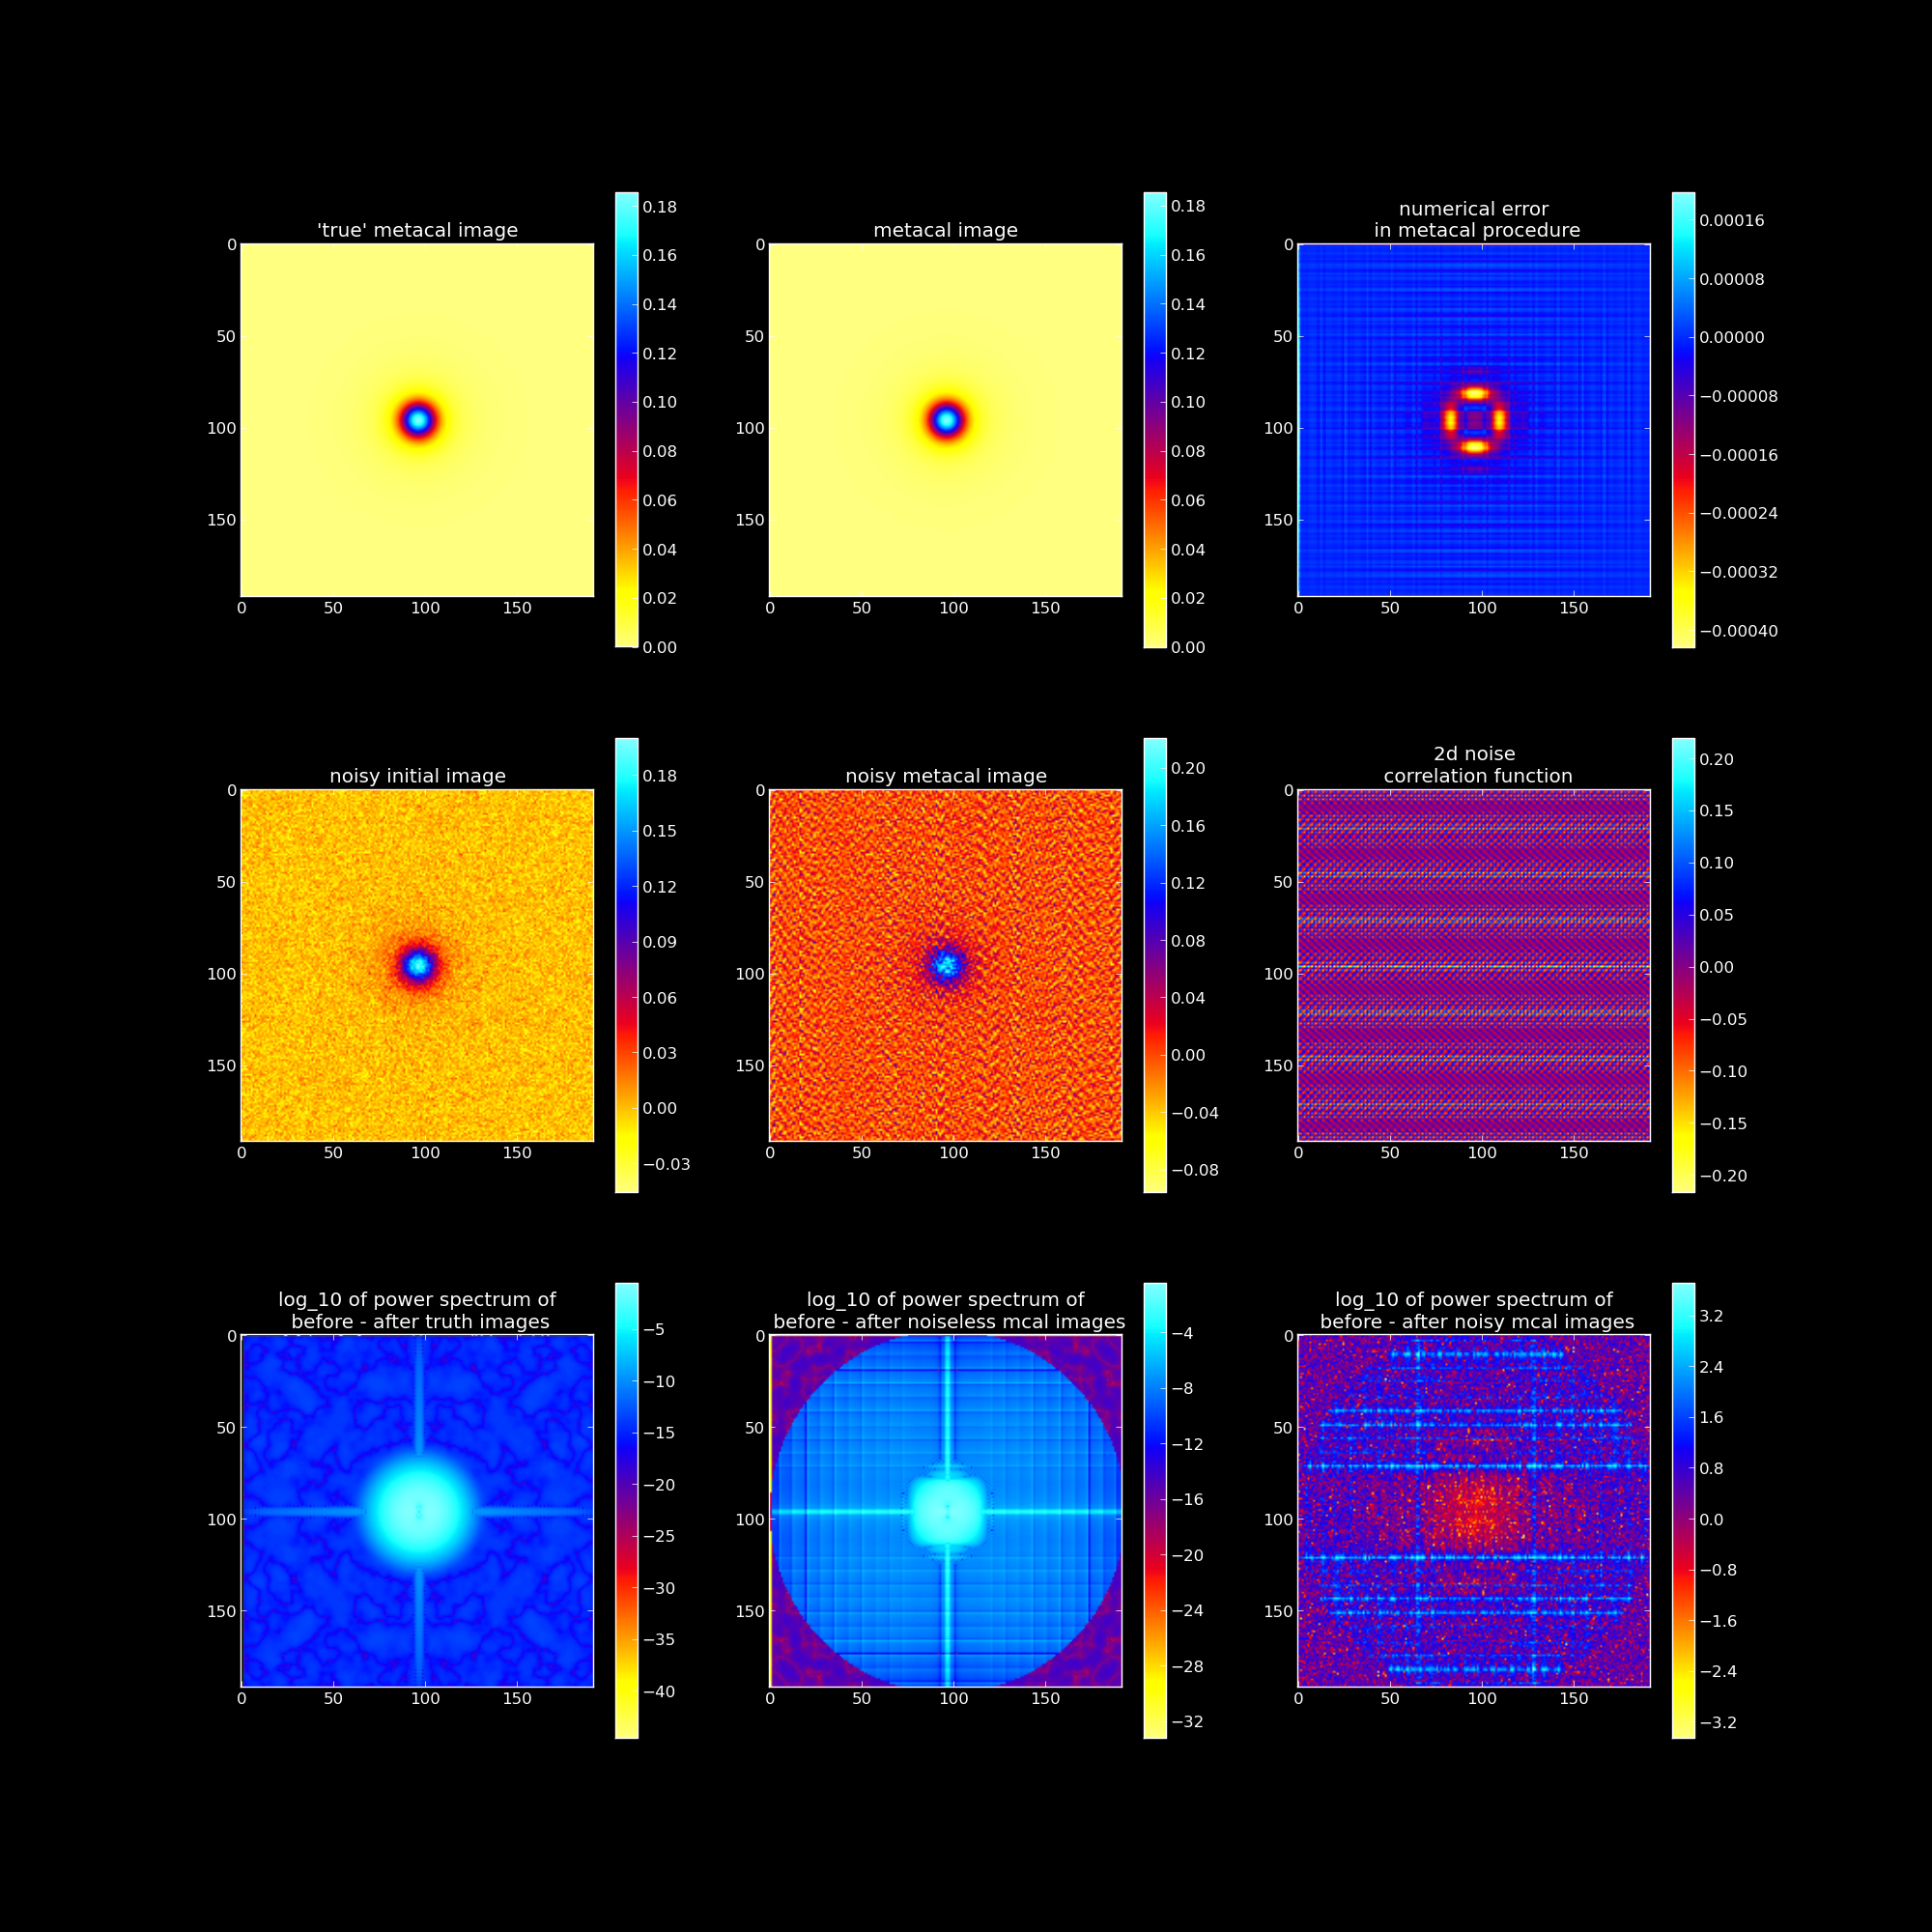
\includegraphics[width=0.75\textwidth]{metacal_noise_images_neg.png}
    \end{figure}
    Figure: Eric Huff (OSU)
}

\frame
{
    \frametitle{Correlated Noise}


    \begin{itemize}

        \item Cancels from mean estimator
            {\color{lightskyblue}
                \begin{equation}
                    E = \frac{E(+\Delta \gamma) + E(-\Delta\gamma)}{2} \nonumber
                \end{equation}
            }

        \item Does not cancel from $R$
            {\color{gold}
                \begin{equation}
                    R = \frac{E(+\Delta\gamma) - E(-\Delta\gamma)}{2 \Delta \gamma} \nonumber 
                \end{equation}
            }

    \end{itemize}

}




\frame
{
    \frametitle{Old Correction for Correlated Noise}

    \setbeamerfont*{itemize/enumerate body}{size=\large}
    \setbeamerfont*{itemize/enumerate subbody}{parent=itemize/enumerate body}
    \setbeamerfont*{itemize/enumerate subsubbody}{parent=itemize/enumerate body}
 
    \begin{itemize}

        \item Originally I was using deeper data to correct: degrade to the
            noise level of the shallow data, but adding noise {\em after}
            performing metacal convolutions/shear.

        \item Deep data is {\color{brightred} expensive} to acquire

        \item Great care must be taken that the deep data is well matched
            to the shallow data

    \end{itemize}

}


\frame
{
    \frametitle{New Correction for Correlated Noise}

    \setbeamerfont*{itemize/enumerate body}{size=\large}
    \setbeamerfont*{itemize/enumerate subbody}{parent=itemize/enumerate body}
    \setbeamerfont*{itemize/enumerate subsubbody}{parent=itemize/enumerate body}
 
    \begin{itemize}

        \item Corrections can be derived from the shallow data itself

        \item The best idea we have:
            \begin{itemize}

                \item The bias due to correlated noise should scale with the
                    {\color{gold} correlation function} of the noise.
                    This is intuitive, but it also has been derived in general
                    by (Hirata, private communication)

                \item Bias thus scales with the {\color{gold} noise} amplitude squared

                \item Add a little noise and look for scaling, remove trend.

            \end{itemize}
    \end{itemize}

}



\frame
{
    \frametitle{Detrending Correction for Correlated Noise}

    \begin{figure}
        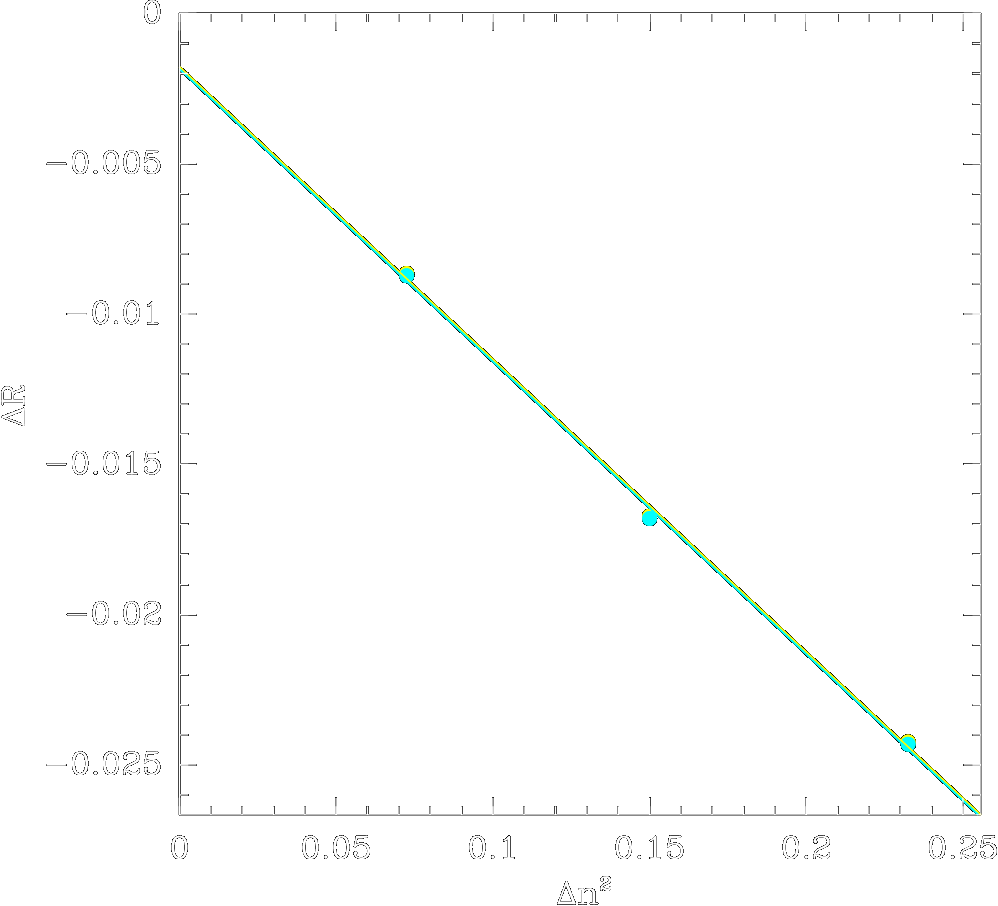
\includegraphics[width=0.65\textwidth]{run-bd13mcal-dt01-Rnoise-detrend-neg.png}
    \end{figure}

    Note offset is not zero
}

\frame
{
    \frametitle{Performance on Simulations}

    \setbeamerfont*{itemize/enumerate body}{size=\large}
    \setbeamerfont*{itemize/enumerate subbody}{parent=itemize/enumerate body}
    \setbeamerfont*{itemize/enumerate subsubbody}{parent=itemize/enumerate body}
 
    \begin{itemize}
        \item Simulations with complex galaxies bulge+disk, with large
            offsets between centers.

        \item Fit a simple gaussian, which normally results in a large ``model bias'',
            of order 10\%.
            
         \item Signal-to-noise ratio $\gtrsim$10, realistic distribution, 
             induces ordinary noise bias of order 10\%

    \end{itemize}

}

\frame
{
    \frametitle{Performance on Simulations}

    \setbeamerfont*{itemize/enumerate body}{size=\large}
    \setbeamerfont*{itemize/enumerate subbody}{parent=itemize/enumerate body}
    \setbeamerfont*{itemize/enumerate subsubbody}{parent=itemize/enumerate body}
 
    \begin{itemize}
            
            
         \item Model the bias as a multiplicative and an additive part
        {\color{lightskyblue} 
            \begin{equation}
                \gamma = (1 + m ) \times \gamma_{true} + c \nonumber
            \end{equation}
        }


         \item With correlated noise corrections

        {\color{gold} 
            \begin{eqnarray}
                m & = & (1.5 \pm 2.0) \times 10^{-3} \nonumber \\
                c & = & (-3.4 \pm 7.0) \times 10^{-5} \nonumber
            \end{eqnarray}
        }
         \item Running now on a larger sim with real galaixes from COSMOS, DES PSF,
            will reach a precision of $\sim 0.7 \times 10^{-3}$

    \end{itemize}

}



\frame
{
    \frametitle{Summary}

    \setbeamerfont*{itemize/enumerate body}{size=\large}
    \setbeamerfont*{itemize/enumerate subbody}{parent=itemize/enumerate body}
    \setbeamerfont*{itemize/enumerate subsubbody}{parent=itemize/enumerate body}
 
    \begin{itemize}
        \item Metacalibration is a new idea for shear recovery from
            Eric Huff

        \item Promising new bias corrections that work {\color{gold} {\em without the need
            for expensive deep data} }

        \item On tests so far, the bias is within statistical error.
        
    \end{itemize}

}

\end{document}
